% Chapter Template

\chapter{Implementation and Results} % Main chapter title

\label{Chapter2} % Change X to a consecutive number; for referencing this chapter elsewhere, use \ref{ChapterX}

%----------------------------------------------------------------------------------------
%	SECTION 1
%----------------------------------------------------------------------------------------

\section{Implementation}
The code base worked with, was a direct Fortran90 implementation of the fingerprint algorithm proposed by \cite{Zhu2016}. The compiler used for all computation was the GNU Fortran compiler \cite{gnufortran}.

\subsection{Data}
The data used were CNSTRUCTURES TODO with either 8 atoms per cell for \emph{training} and 16 atoms per cell for evaluation. The data was gathered by ... for ... . 

\begin{figure}[p]
\center
\label{fig:structures}
\subfloat[8 atom unit cell]{%
  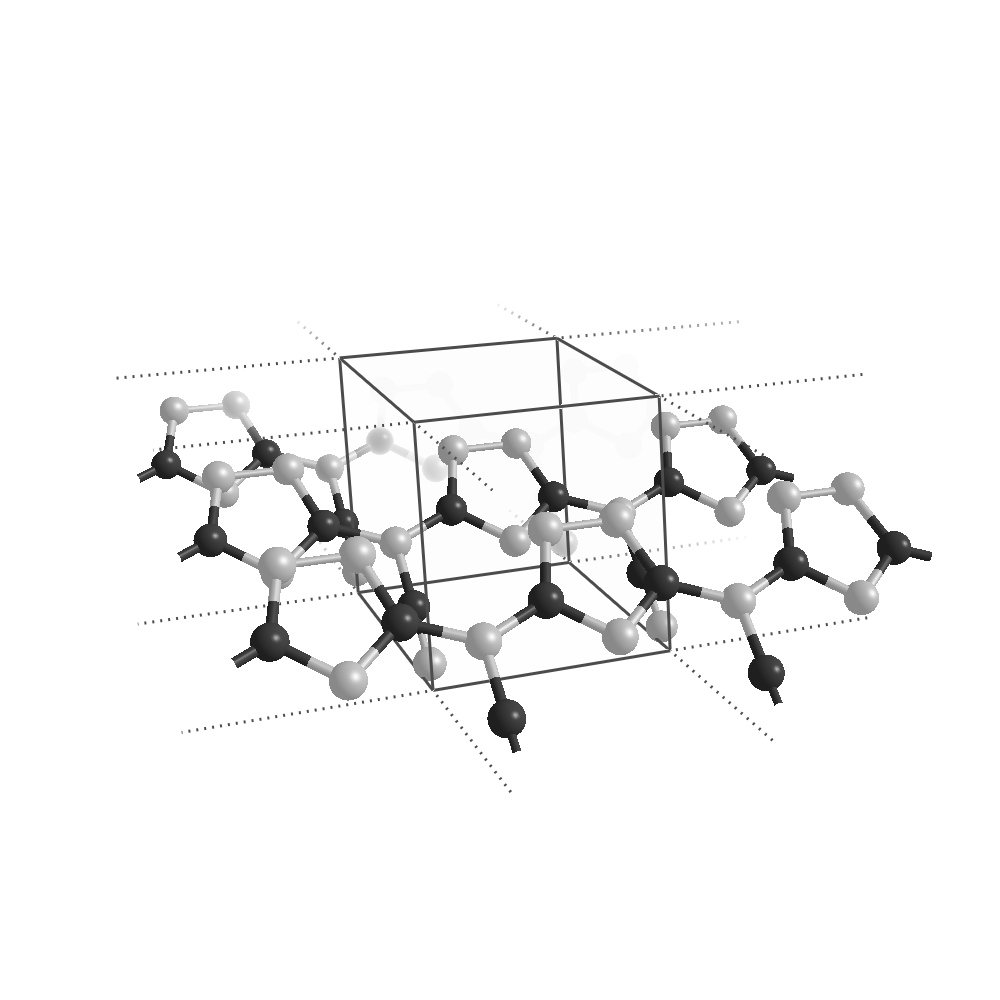
\includegraphics[clip,scale=0.3]{Figures/8structure.png}%
}

\subfloat[16 atom unit cell]{%
  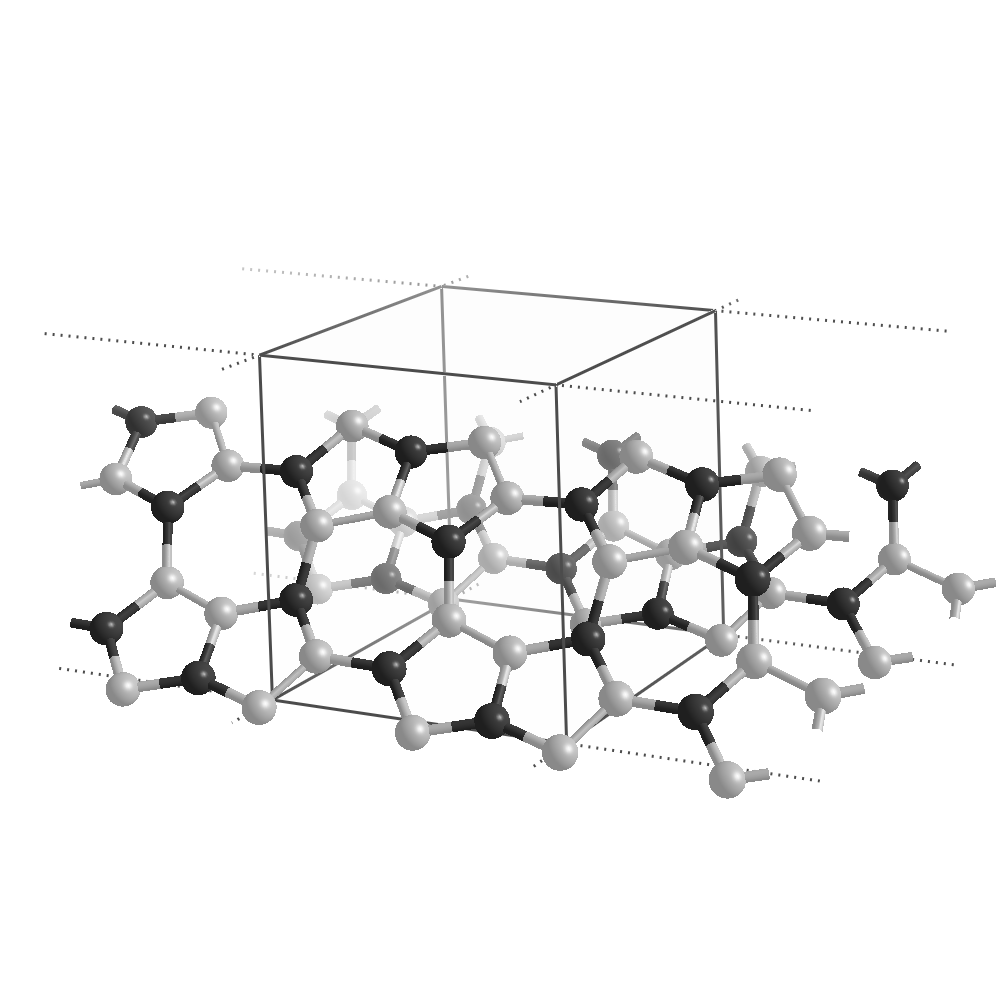
\includegraphics[clip,scale=0.3]{Figures/16structure.png}%
}

\caption{Example of the crystal structures used. C atoms are in black and N atoms in white. (A): Crystal sctructure with 8 atoms per cell. (B): Crystal structure with 16 atoms per cell.}

\end{figure}
\newpage
\subsection{Orbital Energies}
For calculating the overlap matrix (eq. \ref{ovrlap} ff.) the gaussian width $\alpha_i$ was originaly only dependent on the covalent radius of the respective atom type. This was further modified to respect the orbital eigenenergy of the respective orbital (eq. \ref{eq:const}). The values used were gathered from the NIST Atomic Reference Data for Electronic Stucture Calculations.

\begin{table}[h!]
\center
\label{table:energies}
\begin{tabular}{c|c|c}
            & \textbf{C} & \textbf{N} \\ \hline
2s {[}eV{]} & -0.500866  & -0.676151  \\ \hline
2p {[}eV{]} & -0.199186  & -0.266297 
\end{tabular}
\caption{2s and 2p orbital eigenenergies of N and C.}
\end{table}

The constant $C$ in (eq. \ref{eq:const}) was experimentally determined. To obtain a good resolution in comparing the fingerprints, the entries of the fingerprints should be reasonably large, but not to close to each other. One can see the effect of the constant $C$ out of (eq. \ref{eq:const}) by plotting the constant vs. the entries of the fingerprint.
With plots as seen in Figure \ref{fig:const} one can determine approximate boundaries for the constant. The entries should be reasonably distinct but still large enough to get a good resolution. The fine tuning was then done via maximizing the prediction accuracy. The final value used for all calculation was then $C=0.19$.


\begin{figure}[h]

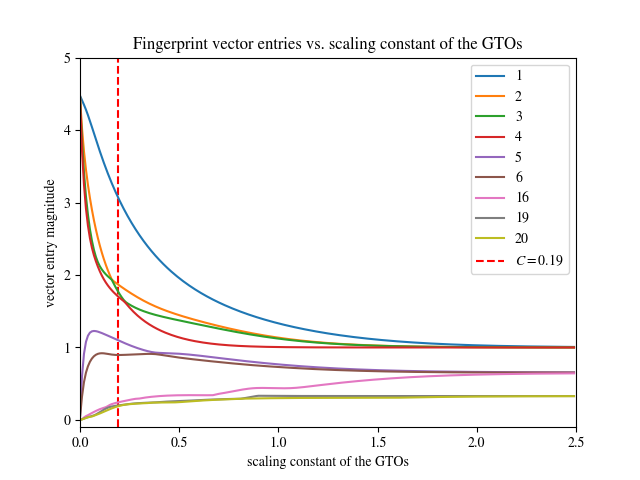
\includegraphics[width=\linewidth]{Figures/fpentry.png}
\caption{Plot of the fingerprint vector entries enumerated vs. the scaling constant of the GTO width.}
\label{fig:const} 
\end{figure}

\newpage
\section{Results}
\subsection{Landmark structures}

To calculate the landmark structures out of the fingerprints, we used a direct implementation of the algorithm maximum volume simplex method \cite{Behnam2020}. The task of this method should be to evaluate all atomar fingerprints given to it, and return the most distinct environments. These most distinct environments should furthermore each describe a different case of possible atomic environment regarding number of nearest neighbours (ligancy or coordination number) and type of nearest neighbours and their permutations. The method was evaluated on the set of 99 crystals with 8 atoms per crystal. Out of these 792 possible environments, the algorithm constructed a maximum volume simplex with 101 corners. A few of these landmark environments can be seen in Figure \ref{fig:landmarks1}, Figure \ref{fig:landmarks2}, Figure \ref{fig:landmarks3} and Figure \ref{fig:landmarks4}. The center atom is always either colored red for carbon and yellow for nitrogen in these depictions. Some of the atomic bonds were omited selectivly for visual clarity.


\begin{figure}[h!]

\center
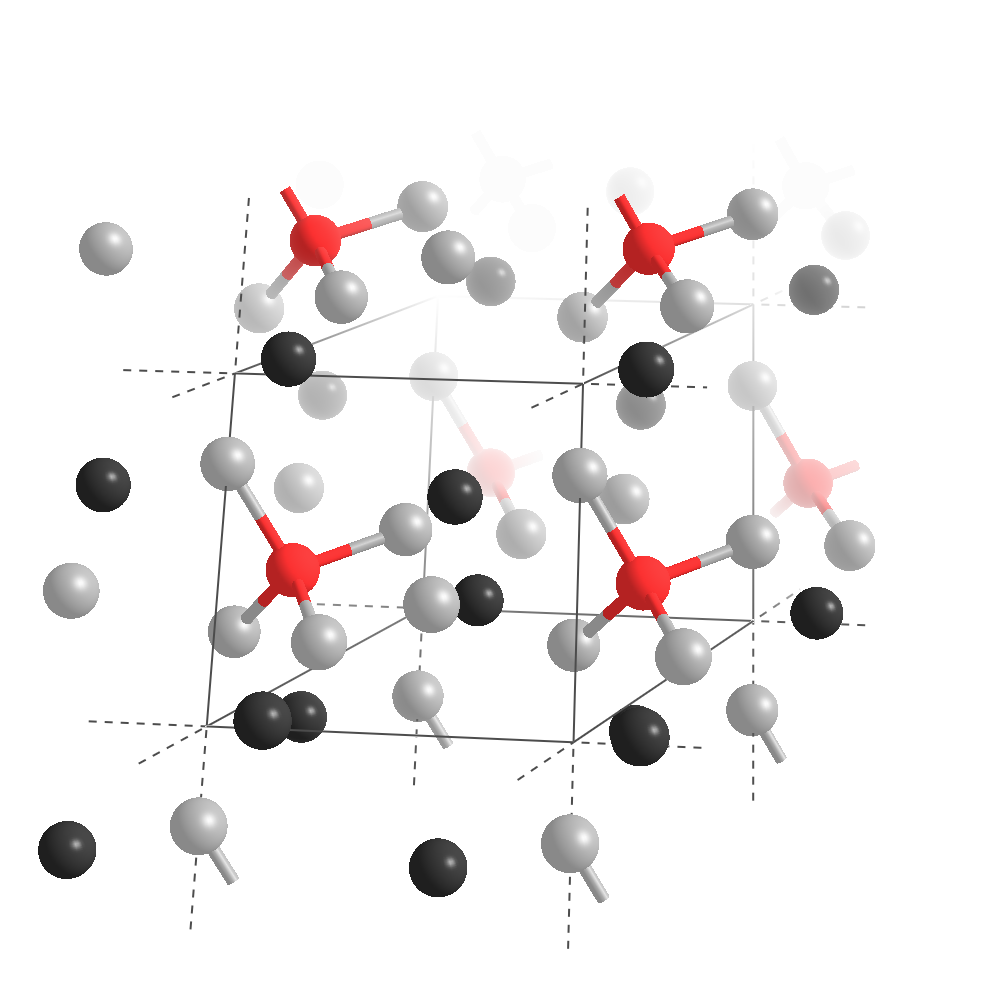
\includegraphics[width=\linewidth]{Figures/landmark1.png}
\caption{Landmark structure: Four times coordinated carbon with 4 nitrogen neighbours; black: carbon; white: nitrogen; red: carbon center atom. }
\label{fig:landmarks1}
\end{figure}

\begin{figure}[p]
\center
\subfloat[One time cooredinated nitrogen]{%
  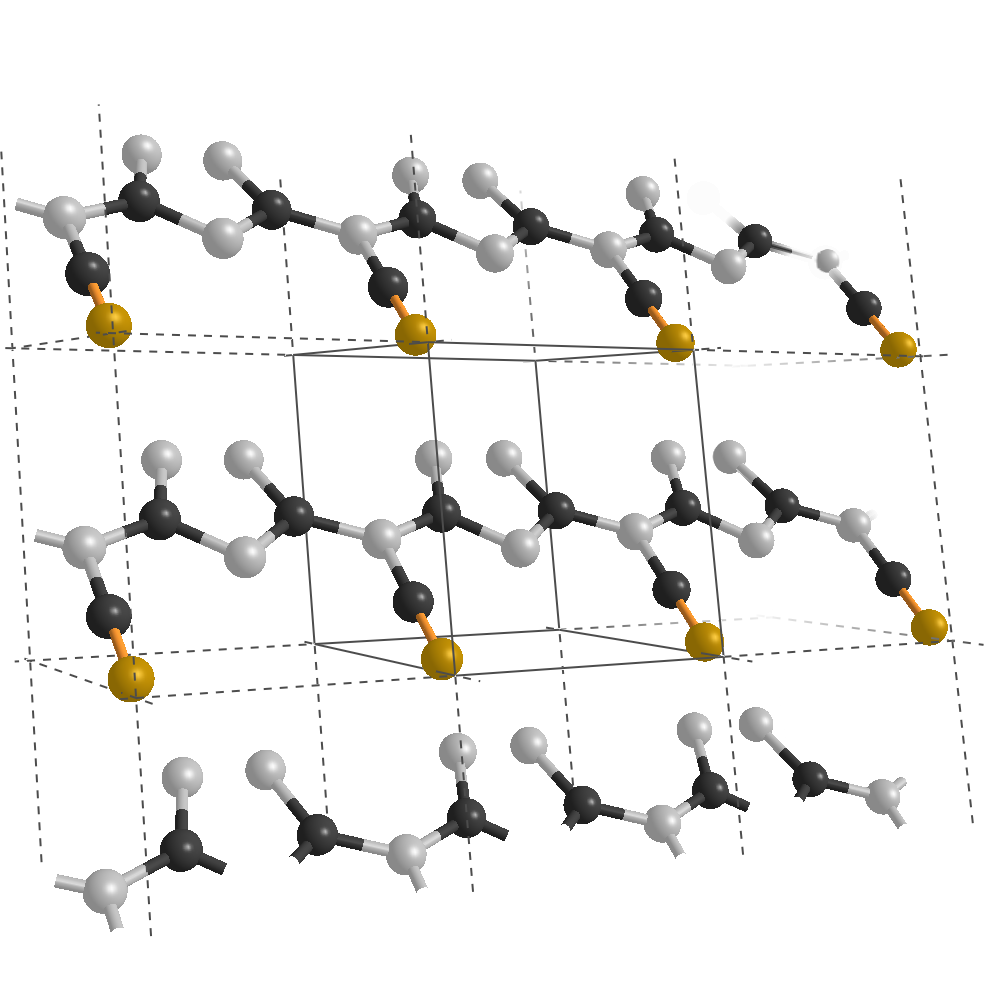
\includegraphics[clip,scale=0.3]{Figures/landmark2.png}%
}

\subfloat[two times coordinated carbon]{%
  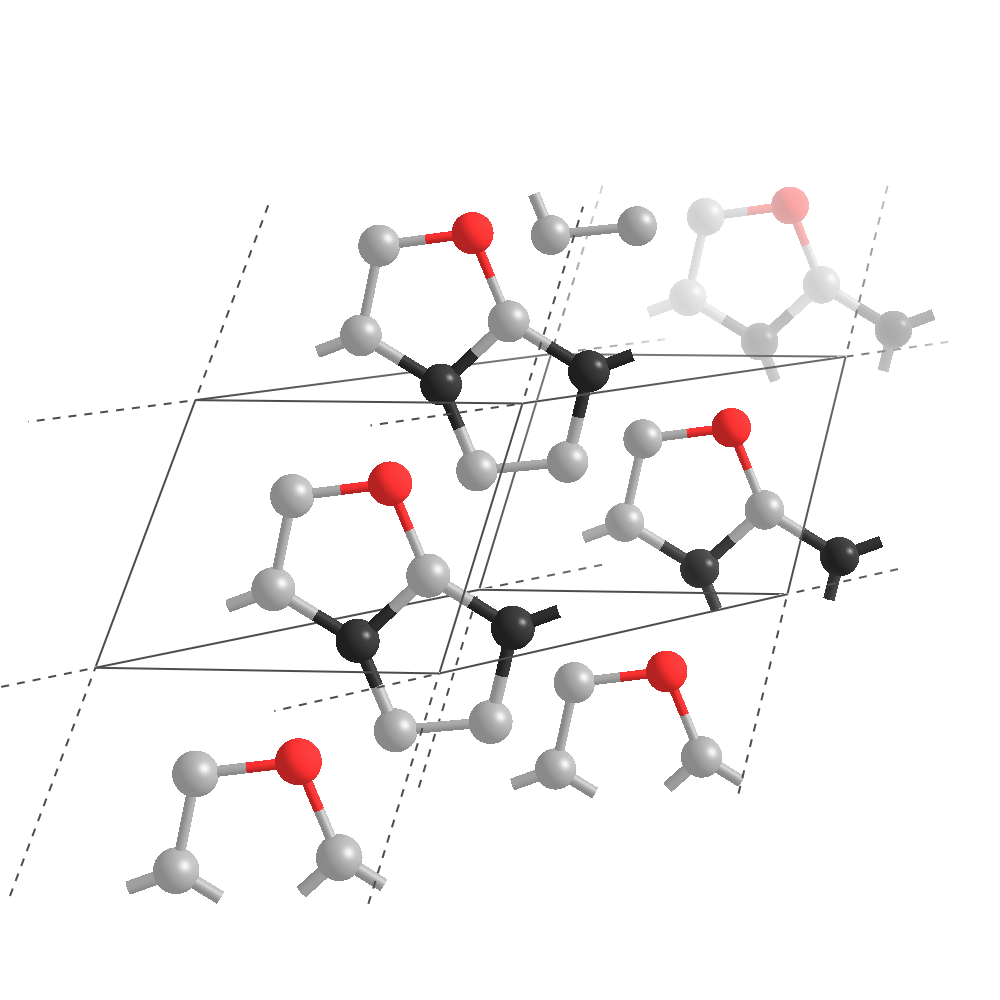
\includegraphics[clip,scale=0.3]{Figures/landmark3.png}%
}

\caption{Landmark structures: black: carbon; white: nitrogen; red: carbon center atom, yellow: nitrogen center atom}
\label{fig:landmarks2}

\end{figure}

\begin{figure}[p]
\center
\subfloat[three times cooredinated nitrogen with 3 carbon and 1 nitrogen neighbour]{%
  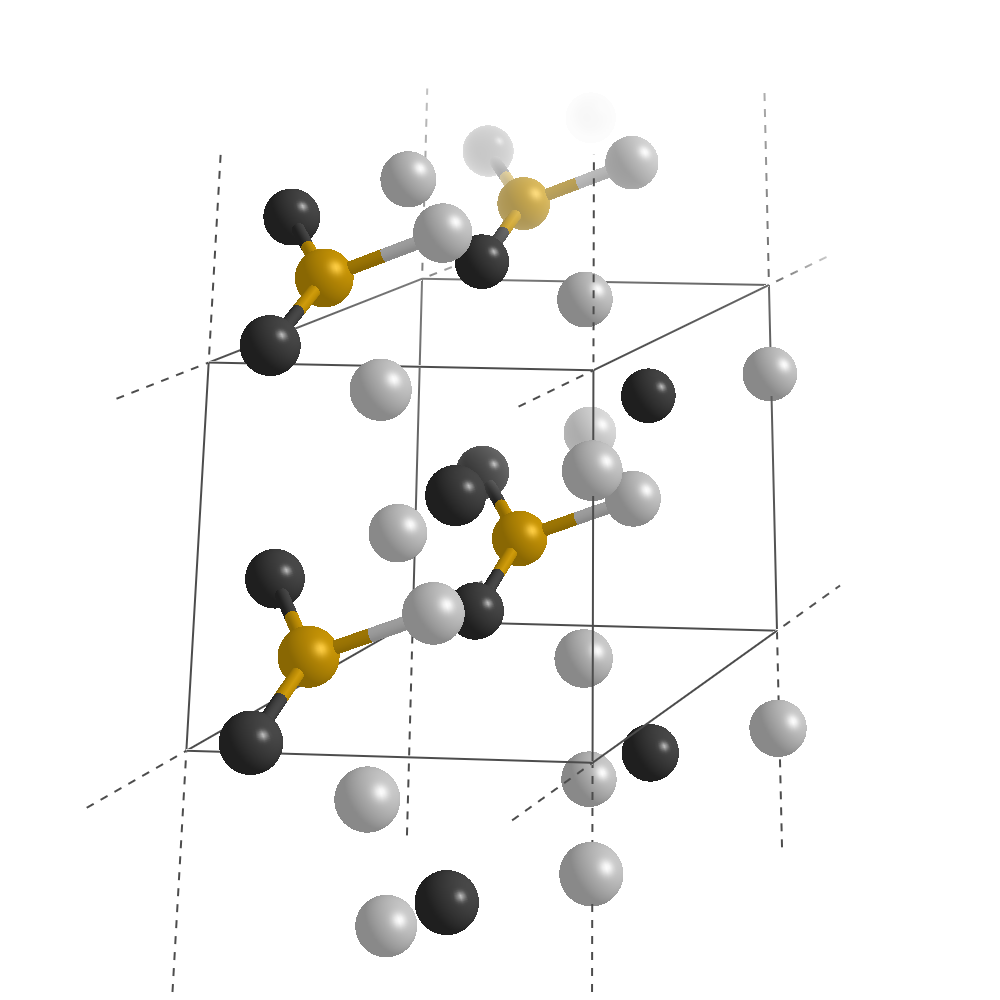
\includegraphics[clip,scale=0.3]{Figures/landmark4.png}%
}

\subfloat[three times cooredinated nitrogen with 3 carbon neighbours]{%
  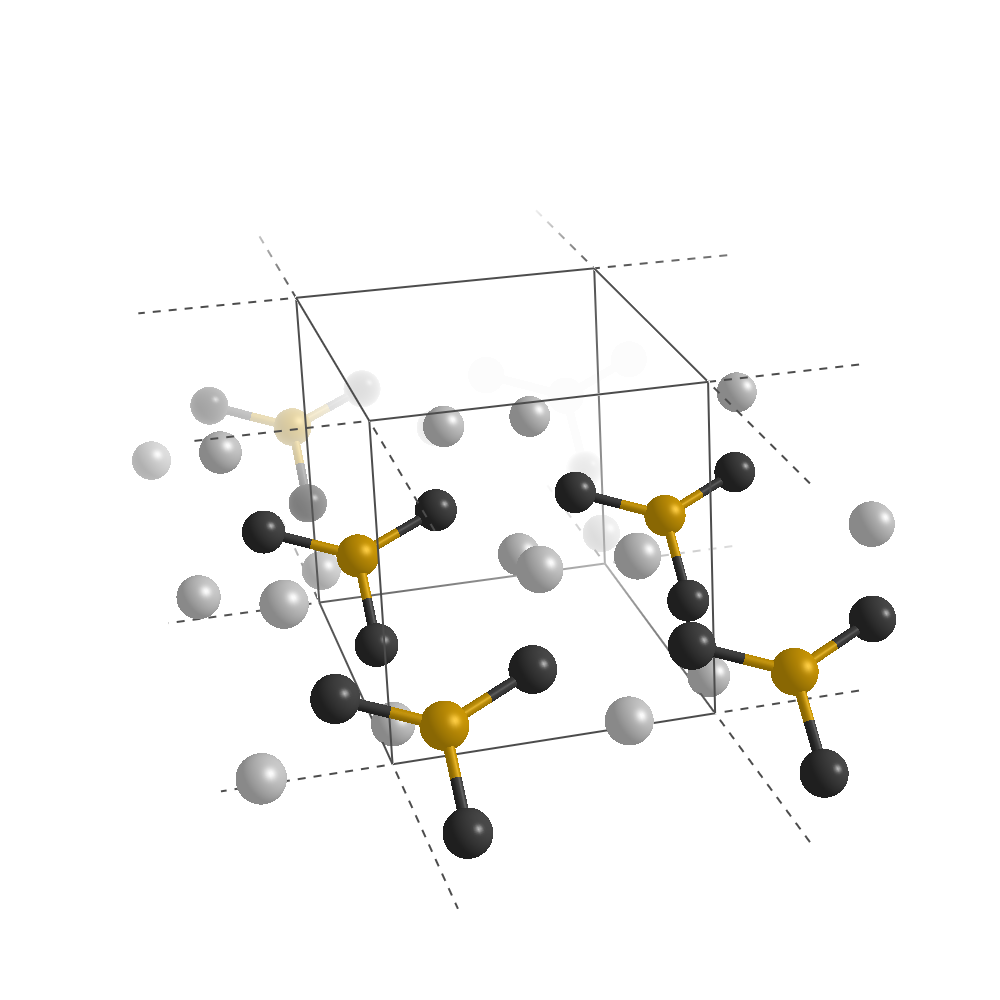
\includegraphics[clip,scale=0.3]{Figures/landmark5.png}%
}

\caption{Landmark structures: black: carbon; white: nitrogen; red: carbon center atom, yellow: nitrogen center atom}
\label{fig:landmarks3}

\end{figure}

\begin{figure}[p]
\center
\subfloat[two times coordinated carbon with 2 nitrogen neighbours]{%
  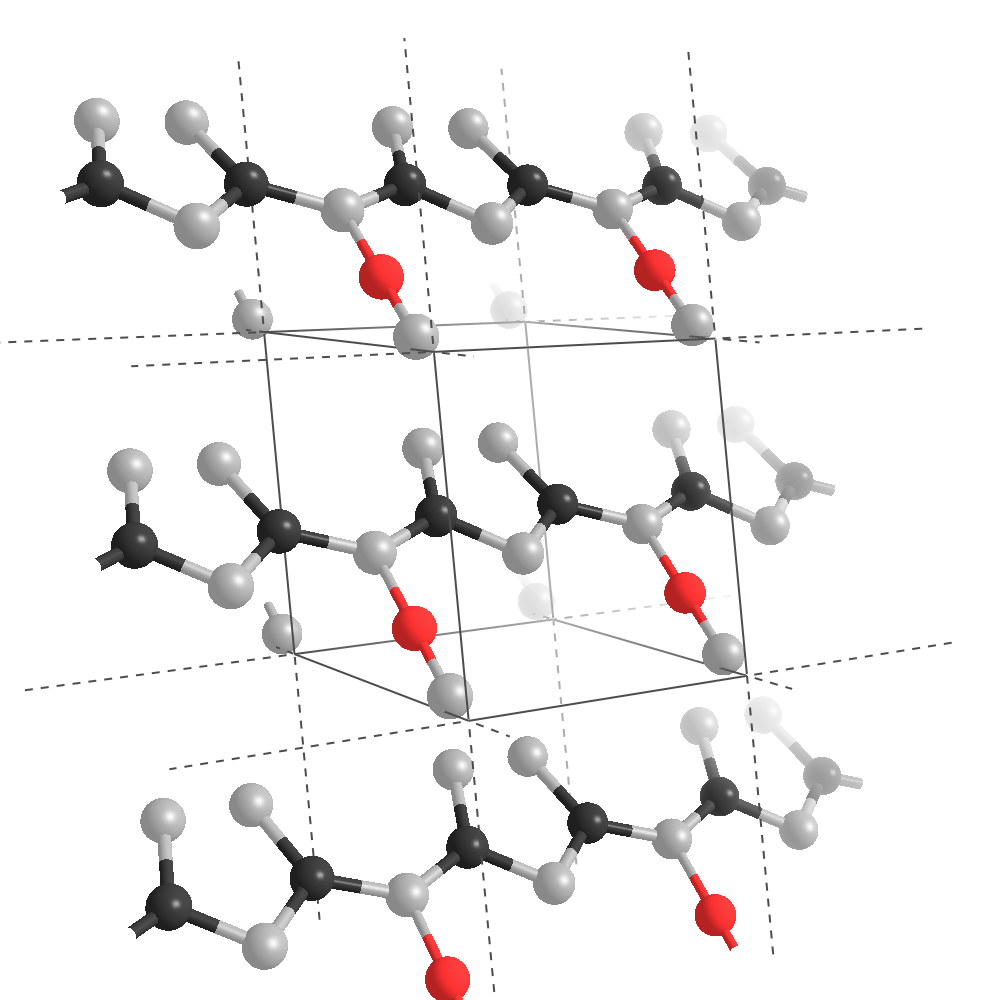
\includegraphics[clip,scale=0.3]{Figures/landmark6.png}%
}

\subfloat[three times cooredinated carbon with 3 nitrogen neighbours]{%
  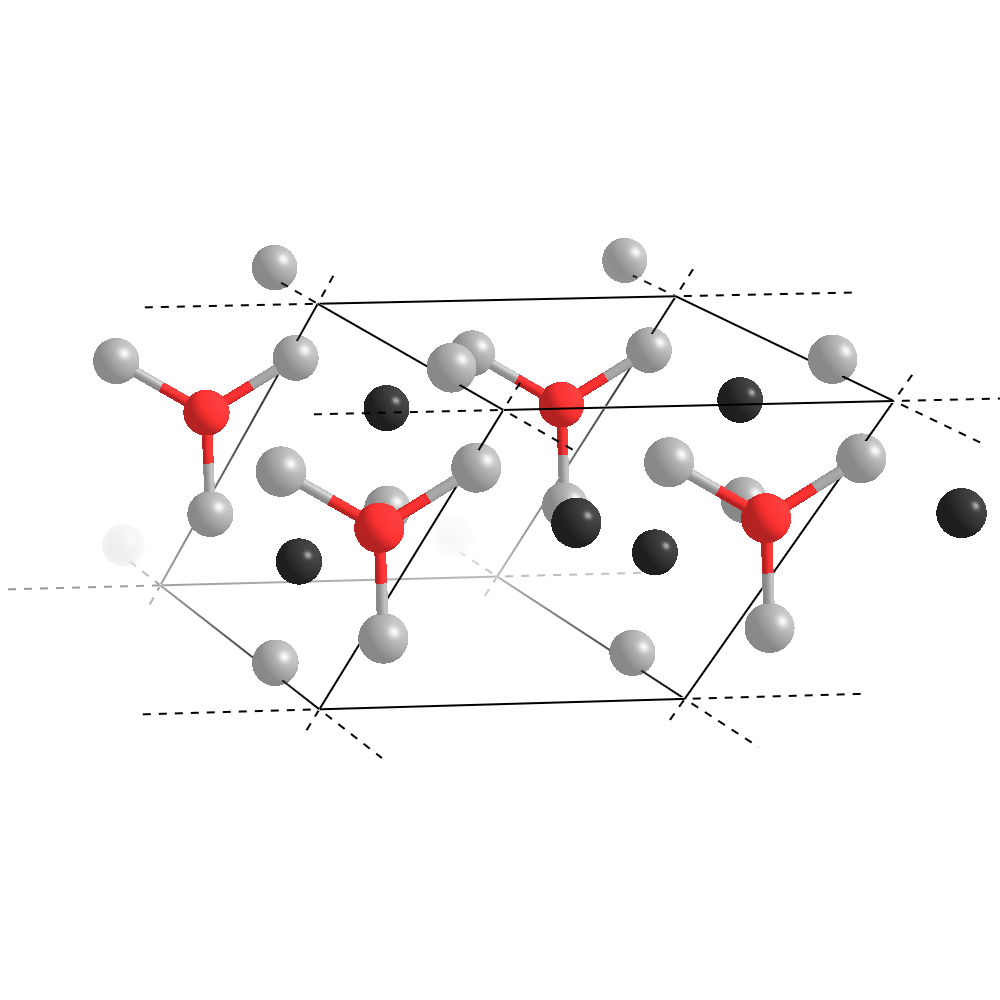
\includegraphics[clip,scale=0.3]{Figures/landmark7.png}%
}

\caption{Landmark structures: black: carbon; white: nitrogen; red: carbon center atom, yellow: nitrogen center atom}
\label{fig:landmarks4}

\end{figure}


\newpage
\subsection{Classification}
The classification was done in a relativly simple way. First, the \emph{trainings fingerprints} are calculated with the procedures mentioned earlier in this text. Then, the maximum simplex method is used to identify 101 landmark fingerprints. Of these landmark fingerprints, the respective center atom is stored aswell. Now, any atomar fingerprint can be compared to the landmark fingerprint via the euclidian distance. If the closest corner to our atom is a carbon, we predict a carbon. If the closest corner is a Nitrogen, we predict a nitrogen.\\
\subsubsection{Training on eight atom crystals}
We trained our model first on a set of 99 configurations with 8 atoms per cell (3 Carbon and 5 Nitrogen). This was then validated on a set of 4949 crystals with 16 atoms per cell (6 carbon and 10 nitrogen) which gives us about 79'000 different environments to classify. The results of this procedure can be seen in Table \ref{table:res1}. 

\begin{table}[h!]
\center
\begin{tabular}{c|c|c|c}
classification & correct & false & correct (relative) \\ \hline
C              & 26497   & 4064  & 0.867              \\ \hline
N              & 45426   & 3197  & 0.934              \\ \hline
Total          & 71923   & 7261  & 0.908             
\end{tabular}
\caption{Classification results for the 4949 carbon nitrate crystals with 16 atoms per cell (79184 atoms in total) trained on 99 crystals with 8 atoms per cell.}
\label{table:res1}
\end{table}

One can see in Table \ref{table:res1} that the classification accuracy for carbon is considerably lower than that for nitrogen. The reason for this effect lies probably within the fact, that our trainings data contains about 1.6 times more nitrogen samples than carbon samples. So our model "knows" the nitrogen case better.

\subsubsection{Training on 16 atom crystals}
Next, we trained our model on a random selction of 63 16 atom crystals out of the 4949 crystals at our disposal. Then we classified the whole set of 16 atom crystals. The results can be seen in Table \ref{table:res2}.

\begin{table}[h!]
\center
\begin{tabular}{c|c|c|c}
classification & correct & false & correct (relative) \\ \hline
C              & 21151   & 3917  & 0.844              \\ \hline
N              & 45573   & 8543  & 0.842              \\ \hline
Total          & 66724   & 12460  & 0.843             
\end{tabular}
\caption{Classification results for the 4949 carbon nitrate crystals with 16 atoms per cell (79184 atoms in total) trained on 63 crystals with 16 atoms per cell.}
\label{table:res2}
\end{table}

Surprisingly, the accuracy is worse than before. Apparently training on a different (smaller) number of atoms per cell yielded better results than on training on the same. This of course can't be taken at face value since evaluating and comparing performance of machine learning methods is a very involved process which we will not get into in this report.

% Training set size: 52789
% Validation set size: 26395
% (79184,)
% (79184, 400)
% [Parallel(n_jobs=1)]: Using backend SequentialBackend with 1 concurrent workers.
% [Parallel(n_jobs=1)]: Done 500 out of 500 | elapsed:  3.1min finished
% [Parallel(n_jobs=1)]: Using backend SequentialBackend with 1 concurrent workers.
% [Parallel(n_jobs=1)]: Done 500 out of 500 | elapsed:    3.2s finished
% The ratio of correct guesses is: 0.9227475941501857
% [[ 8316  1610]
%  [  429 16039]]